\documentclass[10pt,twocolumn,letterpaper]{article}
\usepackage{cvpr}
\usepackage{times}
\usepackage{epsfig}
\usepackage{amsmath}
\usepackage{amssymb}
\usepackage{booktabs} % for much better looking tables
\usepackage{array} % for better arrays (eg matrices) in maths
\usepackage{paralist} % very flexible & customisable lists (eg. enumerate/itemize, etc.)
\usepackage{verbatim} % adds environment for commenting out blocks of text & for better verbatim
\usepackage{subfigure} % make it possible to include more than one captioned figure/table in a single float
\usepackage{graphicx}
\usepackage{multirow}
% Include other packages here, before hyperref.
% If you comment hyperref and then uncomment it, you should delete
% egpaper.aux before re-running latex.  (Or just hit 'q' on the first latex
% run, let it finish, and you should be clear).
%\usepackage[pagebackref=true,breaklinks=true,letterpaper=true,colorlinks,bookmarks=false]{hyperref}
\cvprfinalcopy % *** Uncomment this line for the final submission
\def\cvprPaperID{****} % *** Enter the CVPR Paper ID here
\def\httilde{\mbox{\tt\raisebox{-.5ex}{\symbol{126}}}}
% Pages are numbered in submission mode, and unnumbered in camera-ready
\ifcvprfinal\pagestyle{empty}\fi
\usepackage{url}

%use \x, \y, and \w for bold vector forms
%\newcommand{\x}{\bold{x}}
\DeclareMathOperator*{\argmax}{arg\,max}

\begin{document}
%%%%%%%%% TITLE
\title{
Project in CSE 250B\\
Assignment 4: Latent Dirichlet allocation models with Gibbs sampling}
\author{Andreas Landstad, Spencer Bliven, Jonas Hoelzler\\
Computer Science Department\\
University of California, San Diego\\
{\tt\small landstad.andreas@gmail.com, sbliven@ucsd.edu, jonas@hoelzler.de}
}% For a paper whose authors are all at the same institution,
% omit the following lines up until the closing ``}''.
% Additional authors and addresses can be added with ``\and'',
% just like the second author.
% To save space, use either the email address or home page, not both
%\and
%Second Author\\
%Institution2\\
%First line of institution2 address\\
%{\tt\small secondauthor@i2.org}
\maketitle
\thispagestyle{empty}
%%%%%%%%% ABSTRACT
\begin{abstract}
This project applies latent Dirichlet allocation (LDA) via Gibbs sampling to two data sets. It is applied to a document data set and to a genome data set on the field of bio informatics. For the document data set, 96.50 \% of the documents could be assigned to the correct topic.

\end{abstract}
%%%%%%%%% BODY TEXT


\section{Introduction}
Latent Dirichlet allocation (LDA) is a generative process that can be used for modeling documents in order to find similarities between documents and within documents. This can be useful for clustering them, identifying categories within them or classifying them. In this paper we have used two training sets: Set 1, a set of documents with words and a set of topics to which the documents belong to. Set 2, a set of  genomes with sequences of proteins and organisms to which these sequences belong to. The organisms can in this sense be thought of as topics and the proteins as words. By drawing topic distributions, $\phi_k$, according to the Dirichlet prior $\beta$ and then drawing a distribution over the words $\theta$ according to the Dirichlet prior $\alpha$, LDA is using these two drawn multinomials to draw a topic according to $\theta$ and and then a word according to $\phi_k$. In this way the parameter vectors for topics and words are learned. By using collapsed Gibbs sampling as we have however, the the parameters $\phi$ and $\theta$ are not learned directly, but are instead hidden under parameters $z_i$ belonging to each word. Thus we are learning an estimated $p(z=j|z_j,w_i)$ for each word $i$ and topic $j$.

\subsection{Latent Dirichlet allocation}
For LDA a document is seen as a bag of words with no information about word order. We have a fixed vocabulary $V$ of all words that appear once in a document. Each document can then be represented as a vector of counts for each of these words. One word can appear within different topics and different documents can include words belonging to different topics. Because of this it is the different proportions of each of the topics for one document that is interesting for LDA. It is natural to represent the distribution of topics and words as multinomials, and this is why LDA uses a Dirichlet distribution. 

The Dirichlet distribution is the conjugate prior for multinomial distributions, and LDA uses one Dirichlet distribution with parameter $\alpha$ as prior for the document distribution, and one with parameter $\beta$ for the per-topic word distribution. These parameters could be optimized by grid searching through the $\alpha$s and $\beta$s in order to maximize:

\begin{equation}
p(\bar{w};\alpha,\beta) = \frac{n!}{\prod_{x=1}^{W} \bar{w}_x!} \prod_{x=1}^{V} p(w_i=v|\alpha,\beta)^{\bar{w}_x}
\end{equation}
where $p(w_i=A|\alpha,\beta)=\sum_{j}^{}p(w_i=A,z_i=j)=\sum_{j}\theta_j\phi_{jA}$.
When the $\alpha$ and $\beta$ is fixed, the generative process is as follows:

\begin{itemize}
\item for each topic $j$ 
\begin{itemize}
\item draw a multinomial $\phi_j$ according to $\beta$
\end{itemize}
\item for each document 
\begin{itemize}
\item draw a multinomial $\theta$ according to $\alpha$
\end{itemize}
\begin{itemize}
\item for each word $i$ in the document
\begin{itemize}
\item draw a topic $z$ according to $\theta$
\item draw a word according to $\phi_z$
\end{itemize}
\end{itemize}
\end{itemize}

\subsection{Gibbs sampling}
As mentioned, by using collapsed Gibbs sampling for learning, we don�t actually draw the multinomials $\theta$ and $\phi$ directly. Instead we have a hidden $z$ value for each appearance of each word in the training set. By drawing these $z$�s, Gibbs sampling converges to a distribution of $z$-values for every word. If $\bar{w}�$ is the entire corpora $\bar{w}$ with the word i removed, $\bar{w}\prime$=$\{w_i,\bar{w}\prime\}$ and $\bar{z}$=$\{z_i,\bar{z}\prime\}$, Gibbs sampling works as follows:
\begin{itemize}
\item Take an arbitrary guess $\langle z_1,...,z_n\rangle$
\item Until convergence:
\begin{itemize}
\item	for each word $i$
\begin{itemize}
		\item
Draw $z_i$ according to $p(z_i|\bar{z}\prime_i,\bar{w})$
	\end{itemize}
\end{itemize}
\end{itemize}

In other words we need:
\begin{equation}
p(z_i|\bar{z}�,\bar{w})=
\frac{p(\bar{z},\bar{w})}
{p(\bar{z}\prime,\bar{w})}=
\frac{p(\bar{w}|\bar{z})p(\bar{z})}
{p(w_i|\bar{z}\prime)p(\bar{w}\prime|\bar{z}\prime)p(\bar{z}�)}
\end{equation}
Which yields:
\begin{equation*}
p(z_i=j|\bar{z}\prime,\bar{w})\propto (\frac{q\prime_{j,w_i}+\beta_{w_i}}{\sum_{t=1}^{V}q\prime_{j_t}+\beta_t}) (\frac{n\prime_{mj}+\alpha_j}{\sum_{k=1}^{K}n\prime_{mk}+\alpha_k})
\end{equation*}

\section{Implementation}
LDA gibbs sampling was implemented in Matlab adapted from \cite{heinrich }{Fig. 8}.

 $n_{m,j}$, the count of how many words within document $m$ are assigned to topic $j$, is implemented as a $m$ x $j$ table. $\sum_{k=1}^{K} n_{m,k}$ is the sum of the rows and saved as a $m$ x $1$ array. It stores, how many words one document has.

$q_{m,i}$ is a $m$ x $K$ table storing the current assignment of topics to each appearance
of the word i throughout the corpus. $\sum_{t} q_{j,t}$ stores the sum of all words assigned to one topic stored in a $1$ by $K$ array.

The $z$ values were first chosen randomly and stored in a $m$ x $i$ x $K$ table. The  initial values for the tables explained above were calculated as well.

To get the values for equation 5, the values $w_{m,i}$ for the current assignment $j$ in the table were decremented by one.

Then Equation 5 was calculated and the new assignment $j_{new}$ was sampled. 

After that, the values $w_{m,i}$ were incremented again using assignment $j_{new}$.

One epoch took about 20 seconds on the document dataset using  an AMD Turion X2 Ultra Dual Core Notebook-PC with 2.2 Ghz.

\section{Classic400 Data set}
This data set consists of 400 documents over a vocabulary of 6205 words.
It has $K = 3$ topics. The true labels are given.

 The LDA gibbs sampling was run over 344 iterations with $\alpha$=1 and $\beta$ = 0.01. $\beta$ was selected according to \cite{griffiths}. $\alpha$ was selected small to guarantee fast convergence.  After 300 epochs it seemed to have converged to 96.75 \%. The euclidean distance between $\Theta$ and the true labels can be seen in Figure \ref{convergence}. The covergence against the final accuracy value of 96.75\% can be seen in Figure \ref{accuracy}. $\Phi$ shows the contribution in \% of every word to a topic. The ten words with the highest contribution are shown in Table ref{words}. One possible semantic interpretation of the topics could be Medicine, General Science and Aeronautical Engineering. In Figure \ref{simplex} one can see  a visualization of the documents based on the topics of the trained model, in 3D Euclidean space. One can see the underlying simplex lying in the 3D space. One can see some misclassifications. Most classifications are wrong between topic 1 and topic 3, which are not very similar to topic 2. The middle of the simplex is empty, probably due to the small $\alpha$ value, which results in more decisive topic associations (\cite{heinrich}). 

\begin{figure*}[htbp] 
\centering
   \begin{minipage}{10 cm}
   \centering
    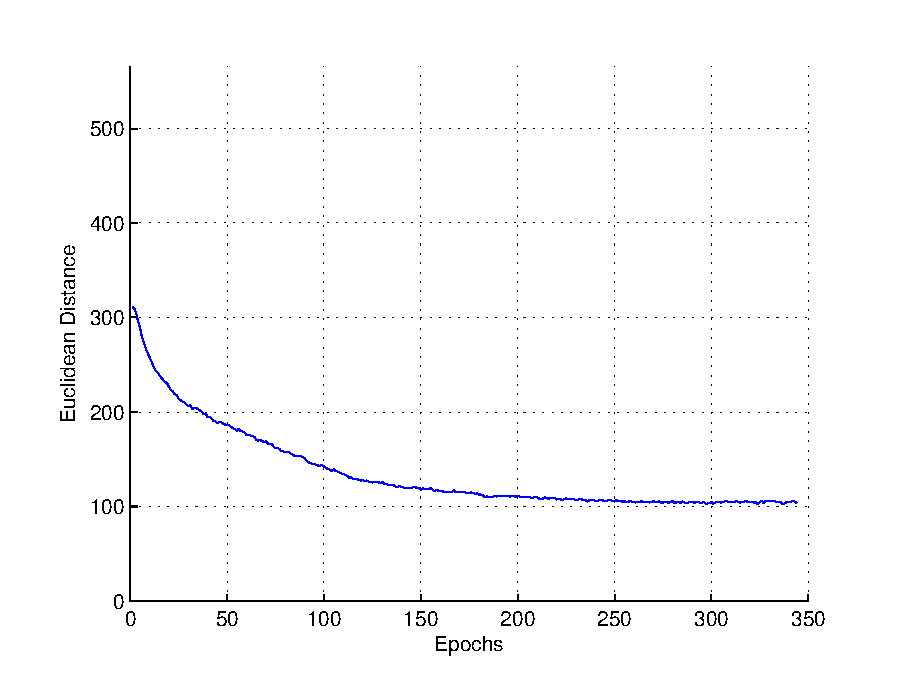
\includegraphics[width=10cm]{images/euclidean}
    \end{minipage}
  \caption{Convergence: Euclidean Distance to simplex of true labels on training on the full classic400 data set}
  \label{convergence}
\end{figure*}

\begin{figure*}[htbp] 
\centering
   \begin{minipage}{10 cm}
   \centering
    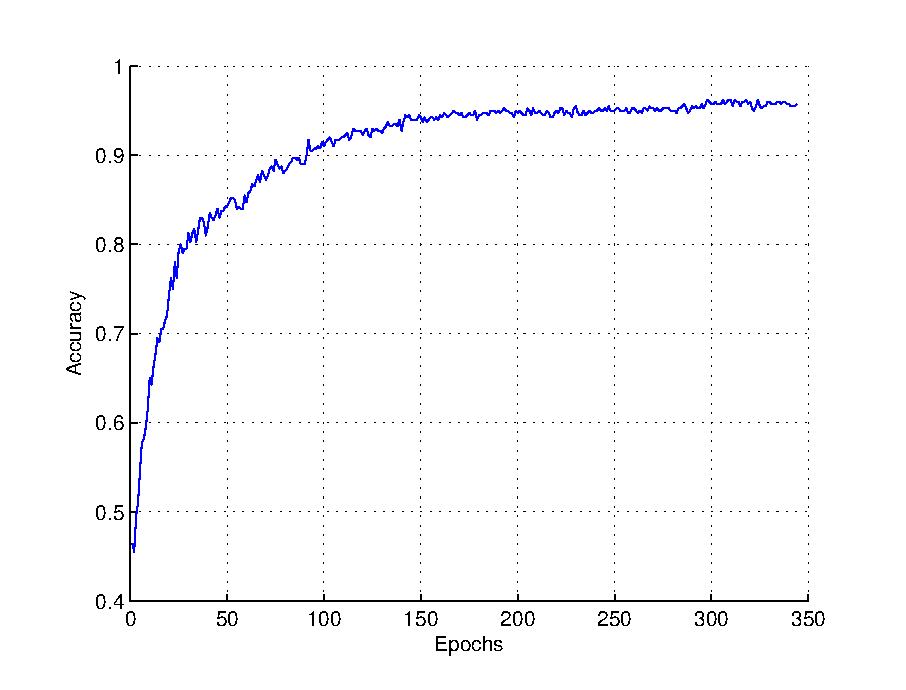
\includegraphics[width=10cm]{images/accuracygrid}
    \end{minipage}
  \caption{Accuracy on training on the full classic400 data set}
  \label{accuracy}
\end{figure*}


\begin{table}
\centering
    \begin{tabular}{|l|l|l|l|}
        \hline
        Rank & Topic 1 & Topic 2 & Topic 3 \\
    		\hline    
			  1 & patients   &   system   &   boundary  \\
			  2 & cases   &   problems   &   layer \\
			  3 & ventricular   &   methods   &   wing  \\
			  4 & fatty   &   research   &   mach  \\
			  5 & left   &   scientific   &   supersonic  \\
			  6 & nickel   &   development   &   ratio\\
			  7 & time   &   retrieval   &   wings \\
			  8 & acids   &   general   &   effects\\
			  9 & aortic   &   part   &   velocity\\
			  10 & free   &   language   &   shock\\
			  \hline
    \end{tabular}
\caption{The words with highest overall $\Phi$ values of the three categories. One possible interpretation of the topics could be Medicine, General Science and Aeronautical Engineering}
\label{words}
\end{table}
%Values
 %   0.0113    0.0083    0.0111
 %   0.0073    0.0069    0.0089
 %   0.0073    0.0067    0.0084
 %   0.0066    0.0065    0.0073
 %   0.0064    0.0063    0.0071
 %   0.0064    0.0059    0.0060
 %   0.0062    0.0058    0.0058
 %   0.0060    0.0055    0.0058
 %   0.0049    0.0049    0.0058
 %   0.0047    0.0048    0.0056



\begin{figure*}[htbp] 
\centering
   \begin{minipage}{10 cm}
   \centering
    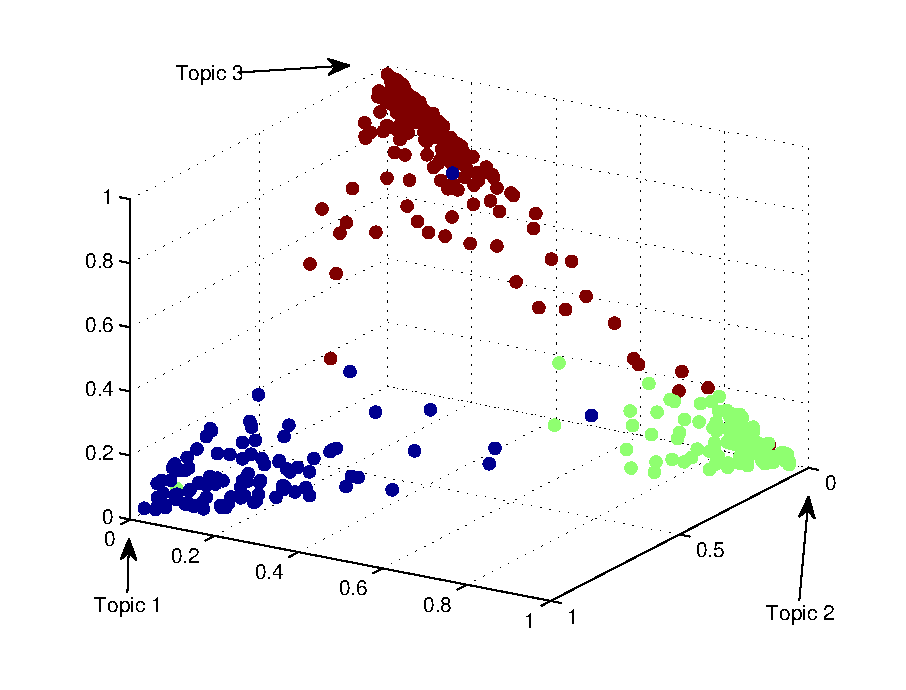
\includegraphics[width=10cm]{images/simplex}
    \end{minipage}
  \caption{Simplex of classic400 training on the full data set.  The colors show the truelabels. There are 13 wrong classifications. Most classifications are wrong between topic 1 and topic 3, which are not very similar to topic 2.}
  \label{simplex}
\end{figure*}

\subsection{Log likelihood of training set}

After estimating $\theta_m$ and $\phi_j$ for a training set, the log likelihood of the training set can be calculated can be calculated. For a each document $\bar{w} = \bar{w}_1,\dots,\bar{w}_V$, the likelihood of that document is
\begin{align}
p(\bar{w};\alpha,\beta) &= \frac{n!}{\prod_{x=1}^{W} \bar{w}_x!} \prod_{x=1}^{V} p(w_i=v_x|\alpha,\beta)^{\bar{w}_x}
\end{align}
where $w_i$ indicates the word at arbitrary position $i$ within a document, and $v_x$ indicates the $x$th word of the vocabulary.
\begin{align}
p(w_i=A|\alpha,\beta)=\sum_{j}^{}p(w_i=A,z_i=j)=\sum_{j}\theta_j\phi_{jA}
\end{align}

The log likelihood of the ten most likely words can be found in Table ref{log}.

\begin{table}
\centering
	\begin{tabular}{|l|l|}
    	\hline
    	Word    	& Log-Likelihood \\ 
    	general 	& 4.7633     	\\ 
    	considered  & 4.7633     	\\ 
    	present 	& 4.7617     	\\
    	based   	& 4.7614     	\\ 
    	shown   	& 4.7612     	\\ 
    	high    	& 4.7609     	\\ 
    	development & 4.7608     	\\ 
    	compared	& 4.7607     	\\ 
    	developed   & 4.7606     	\\ 
    	application & 4.7603     	\\
    	\hline
	\end{tabular}
\caption{Log likelihood of ten most probably words}
\label{log}
\end{table}

\section{Genome Dataset}

Although LDA is couched in terms of words and documents, the LDA model can be extended to any type of information which is expressed as a sequence over some abstract alphabet. To demonstrate this, we encode genomes as sequences of proteins, and use LDA to classify organisms.

The genome of an organism can be thought of as a long sequence of genes. Since closely related genes tend to be functionally similar, genes can be classified into families. One organism may contain several copies of genes from the same family, and a broad range of species may have genes belonging to the same family. Thus, the concept of a �bag of words� representation for text documents can be extended to a �bag of gene families� representation of single genomes. Such a representation was generated for a wide range of genomes and is refered to as the \begin{em}genome dataset\end{em}. 

\subsection{Construction of the Genome Dataset}

%added
%The UniProt Consortium
%Ongoing and future developments at the Universal Protein Resource
%Nucleic Acids Res. 39: D214-D219 (2011).

%add
%Jain E., Bairoch A., Duvaud S., Phan I., Redaschi N., Suzek B.E., Martin M.J., McGarvey P., Gasteiger E.
%Infrastructure for the life sciences: design and implementation of the UniProt website
%BMC Bioinformatics 2009, 10:136.

%           The Pfam protein families database: R.D. Finn, J. Mistry, J. Tate, P. Coggill, A. Heger, J.E. Pollington, O.L. Gavin, P. Gunesekaran, G. Ceric, K. Forslund, L. Holm, E.L. Sonnhammer, S.R. Eddy, A. Bateman Nucleic Acids Research (2010)  Database Issue 38:D211-222


Initially, 1207 species were selected for analysis based on their annotation in UniProt (release 2011\textunderscore 03) \cite{uniprot,jain} as being �complete� and �reviewed and annotated�\footnote{For more information about compete genomes, see \url{http://www.uniprot.org/faq/15}}. All UniProt/Swiss-Prot entries for each species were subsequently downloaded and used to define the genome of each species. Note that the automatically annotated TrEMBL database was not used for performance reasons, although automatic curations would have significantly increased the number of genes considered for some organisms. In total, 525,997 unique genes were considered.

The Pfam database was used to cluster genes into families \cite{finn}. There are 11,912 families in the Pfam database (Pfam A, version 24, Oct 2009), which clusters UniProt proteins into families according to a set of profile hidden Markov models.  429,383 unique matches of protein families were mapped to the genomes, with a duplication within genomes giving a total of 685,267 proteins.


After mapping pfams onto genomes, 141 genomes were discarded due to zero coverage by Pfam. These genomes were likely sequenced after the last update of Pfam in late 2009. 
Out of the 1066 remaning genomes, 81\% were bacterial. This distribution reflects the large amount of bacteria which have been recently sequenced. However, it should be noted that many of the bacteria included are closely related. For instance, 35 strains of \begin{em}E. coli\end{em} have been completely sequenced, do to the importance of this bacteria as a model organism and the relative inexpensiveness of resequencing a bacterial genome.
To account for this bias, 200 bacterial genomes were chosen at random for the dataset.
See figures \ref{fig:eukaryotaTree}--\ref{fig:bacteria2Tree} for a complete list of species concidered. 
Additionally, 3560 Pfam families were discarded because they did not map to any of the species considered. After this filtering, the genome dataset consisted of 400 genomes over a vocabulary of        8352 protein families.

\subsection{Distribution of Genome Dataset}

Out of the 400 genomes considered in the genome dataset, 130 (32\%) came from Eukaryota,    70 (18\%) from Archaea, and    200 (50\%) from Bacteria.

\begin{table*}
\centering
	\begin{tabular}{|l|l|l|}
    	\hline
    	Rank &PFam Accessor    	& Description \\ 
	\hline
	1 & PF00400.25 & WD domain, G-beta repeat \\
	2 & PF00096.19 & Zinc finger, C2H2 type \\
	3 & PF00023.23 & Ankyrin repeat \\ %mostly eukaryotic
	4 & PF07679.9 & Immunoglobulin I-set domain \\ %antibody
	5 & PF00041.14 & Fibronectin type III domain \\ %plasma, wound healing
	6 & PF00001.14 & 7 transmembrane receptor (rhodopsin family) \\ %euk membrane
	7 & PF00028.10 & Cadherin domain \\ %cell adhesion
	8 & PF00076.15 & RNA recognition motif. (a.k.a. RRM, RBD, or RNP domain) \\ %58/60 label 1
	9 & PF00069.18 & Protein kinase domain \\ %SURPRISE! well conserved. Ah, but not in my set. 66/3/31 distribution
	10 & PF00560.26 & Leucine Rich Repeat  \\% 42/0/9
    	\hline
	\end{tabular}
\caption{Ten most probable protein families for Eukaryotes (from $\phi_{\mbox{Eukaryota}}$).}
\label{tab:eukTop10}
\end{table*}

\begin{table*}
\centering
	\begin{tabular}{|l|l|l|}
    	\hline
    	Rank &PFam Accessor    	& Description \\ 
	\hline
	1 & PF01535.13 & PPR repeat \\ %plants? 24/0/0!
	2 & PF00560.26 & Leucine Rich Repeat \\ %42/0/9!
	3 & PF00069.18& Protein kinase domain\\ %66     3    31
	4 & PF00646.26 &  F-box domain \\%ubiquitination 36/0/0
	5 & PF00400.25 & WD domain, G-beta repeat \\% 89     0     2  
	6 & PF00005.20 & ABC transporter \\ % everywhere 34    25   421 
	7 & PF00036.25 & EF hand \\%  signalling and transport 46     0     0 
	8 & PF07714.10 & Protein tyrosine kinase \\%  18     0     0  
	9 &  PF00085.13 & Thioredoxin \\ % 21     0    93 
	10 & PF00642.17 & Zinc finger C-x8-C-x5-C-x3-H type (and similar) \\%  30     0     0 
    	\hline
	\end{tabular}
\caption{Ten most probable protein families for Archaea (from $\phi_{\mbox{Archaea}}$).}
\label{tab:archTop10}
\end{table*}

\begin{table*}
\centering
	\begin{tabular}{|l|l|l|}
    	\hline
    	Rank &PFam Accessor    	& Description \\ 
	\hline
	1 & PF03144.18 & Elongation factor Tu domain 2 \\  % Protein synthesis 82    62   807  
	2 & PF00009.20 & Elongation factor Tu GTP binding domain \\% Protein synth 97    62   807 
	3 & PF00005.20 & ABC transporter \\ % everywhere 34    25   421 
	4 & PF04055.14 & Radical SAM superfamily \\%  diverse specialized reactions �including unusual methylations, isomerization, sulphur insertion, ring formation, anaerobic oxidation and protein radical formation� 75    51   751 
	5 & PF00587.18 & tRNA synthetase class II core domain (G, H, P, S and T) \\%   15    64   808  
	6 & PF01926.16 & GTPase of unknown function
 \\%  19    14   806  
	7 & PF00156.20 & Phosphoribosyl transferase domain \\% nucleotide synth an salvage 26    58   722 
	8 & PF03129.13 & Anticodon binding domain \\% 15    63   800 
	9 & PF00133.15 & tRNA synthetases class I (I, L, M and V) \\%  14    48   740  
	10 & PF00006.18 & ATP synthase alpha/beta family, nucleotide-binding domain \\%26    61   783 
    	\hline
	\end{tabular}
\caption{Ten most probable protein families for Bacteria (from $\phi_{\mbox{Bacteria}}$).}
\label{tab:bacTop10}
\end{table*}


%	'PF00400.25'	'PF01535.13'	'PF03144.18'
%	'PF00096.19'	'PF00560.26'	'PF00009.20'
%	'PF00023.23'	'PF00069.18'	'PF00005.20'
%	'PF07679.9' 	'PF00646.26'	'PF04055.14'
%	'PF00041.14'	'PF00400.25'	'PF00587.18'
%	'PF00001.14'	'PF00005.20'	'PF01926.16'
%	'PF00028.10'	'PF00036.25'	'PF00156.20'
%	'PF00076.15'	'PF07714.10'	'PF03129.13'
%	'PF00069.18'	'PF00085.13'	'PF00133.15'
%	'PF00560.26'	'PF00642.17'	'PF00006.18'


\section{Discussion}








\subsection{Choosing parameters}
We already had a set number of categories and hence did not have to pick the number of topics. This, however, could be interesting as tweaking the amount of topics can cluster new documents together. The number of topics is not a question of maximum likelihood, but more of what you are trying to reveal or what you are trying to classify. The genomes for example, if they had provided better results, could have shown similarities on different levels in the hierarchy. Other parameters that had to be chosen were $\alpha$ and $\beta$. We simply fixed these to $\alpha = 1$ and $\beta=0.01$. $\beta$ was selected according to \cite{griffith}, while alpha was selected smaller than the proposed value from Griffith to get, according to \cite{heinrich} faster more decisive  topic associations. As mentioned however, we could have grid-searched $\alpha$ and $\beta$ in order to find the ones that maximized the likelihood. As always when learning we are in danger of overfitting to the data we are learning from. A way we could have tested for overfitting would have been to use cross validation and measured accuracy by the percent of correct predictions of the test-set.

\begin{figure*}[htbp]
 \centering
 \subfigure[~]{
    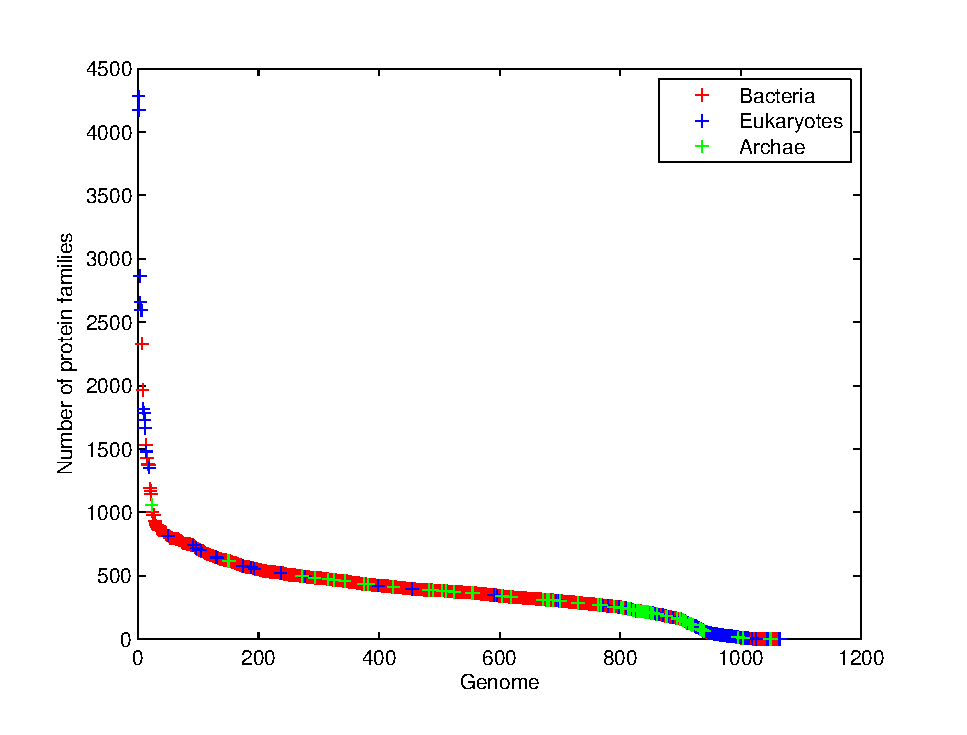
\includegraphics[width=5cm]{images/proteinsPerGenome}
}
   \subfigure[~]{
    \includegraphics[width=5cm]{images/genomesPerProtein}
}
   \caption{(a) Number of protein families per genome. Each Pfam is counted once per genome, and genomes are sorted according to number of unique pfams identified in that species. (b) Number of species per protein family. Each species is counted once per Pfam, and protein families are sorted according to the number of species which have one or more occurances of that family.}
\end{figure*}


\begin{figure*}[htbp] 
\centering
   \begin{minipage}{10 cm}
   \centering
    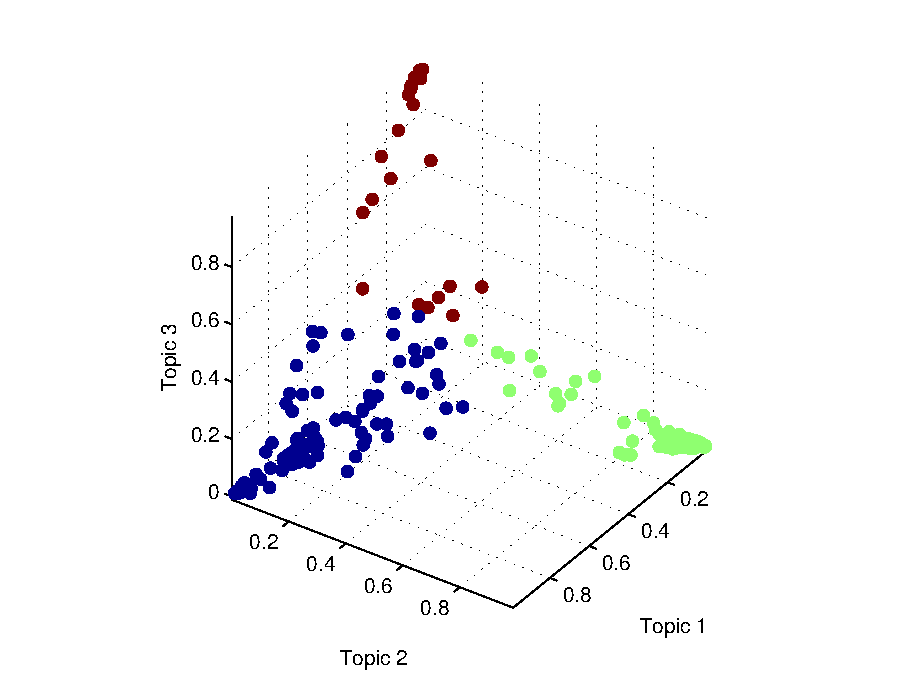
\includegraphics[width=10cm]{images/foundlabelssimplex}
    \end{minipage}
  \caption{foundlabelssimplex}
  \label{foundlabelssimplex}
\end{figure*}

\begin{figure*}[htbp] 
\centering
   \begin{minipage}{10 cm}
   \centering
    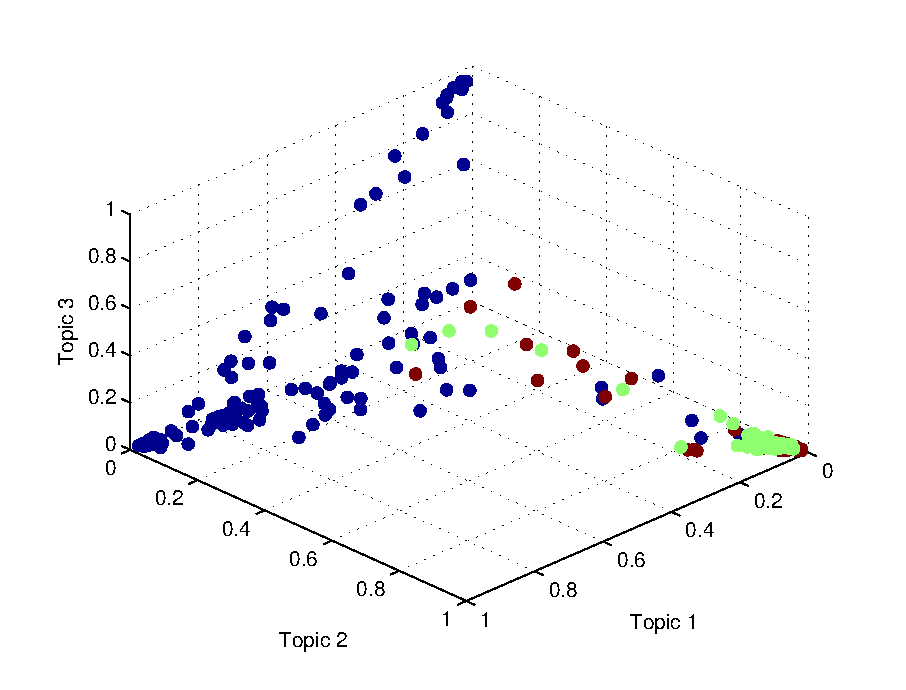
\includegraphics[width=10cm]{images/truelabelssimplex}
    \end{minipage}
  \caption{truelabelssimplex}
  \label{truelabelssimplex}
\end{figure*}






% Long, hard to read phylogenetic trees
\begin{figure*}[p] 
\centering
    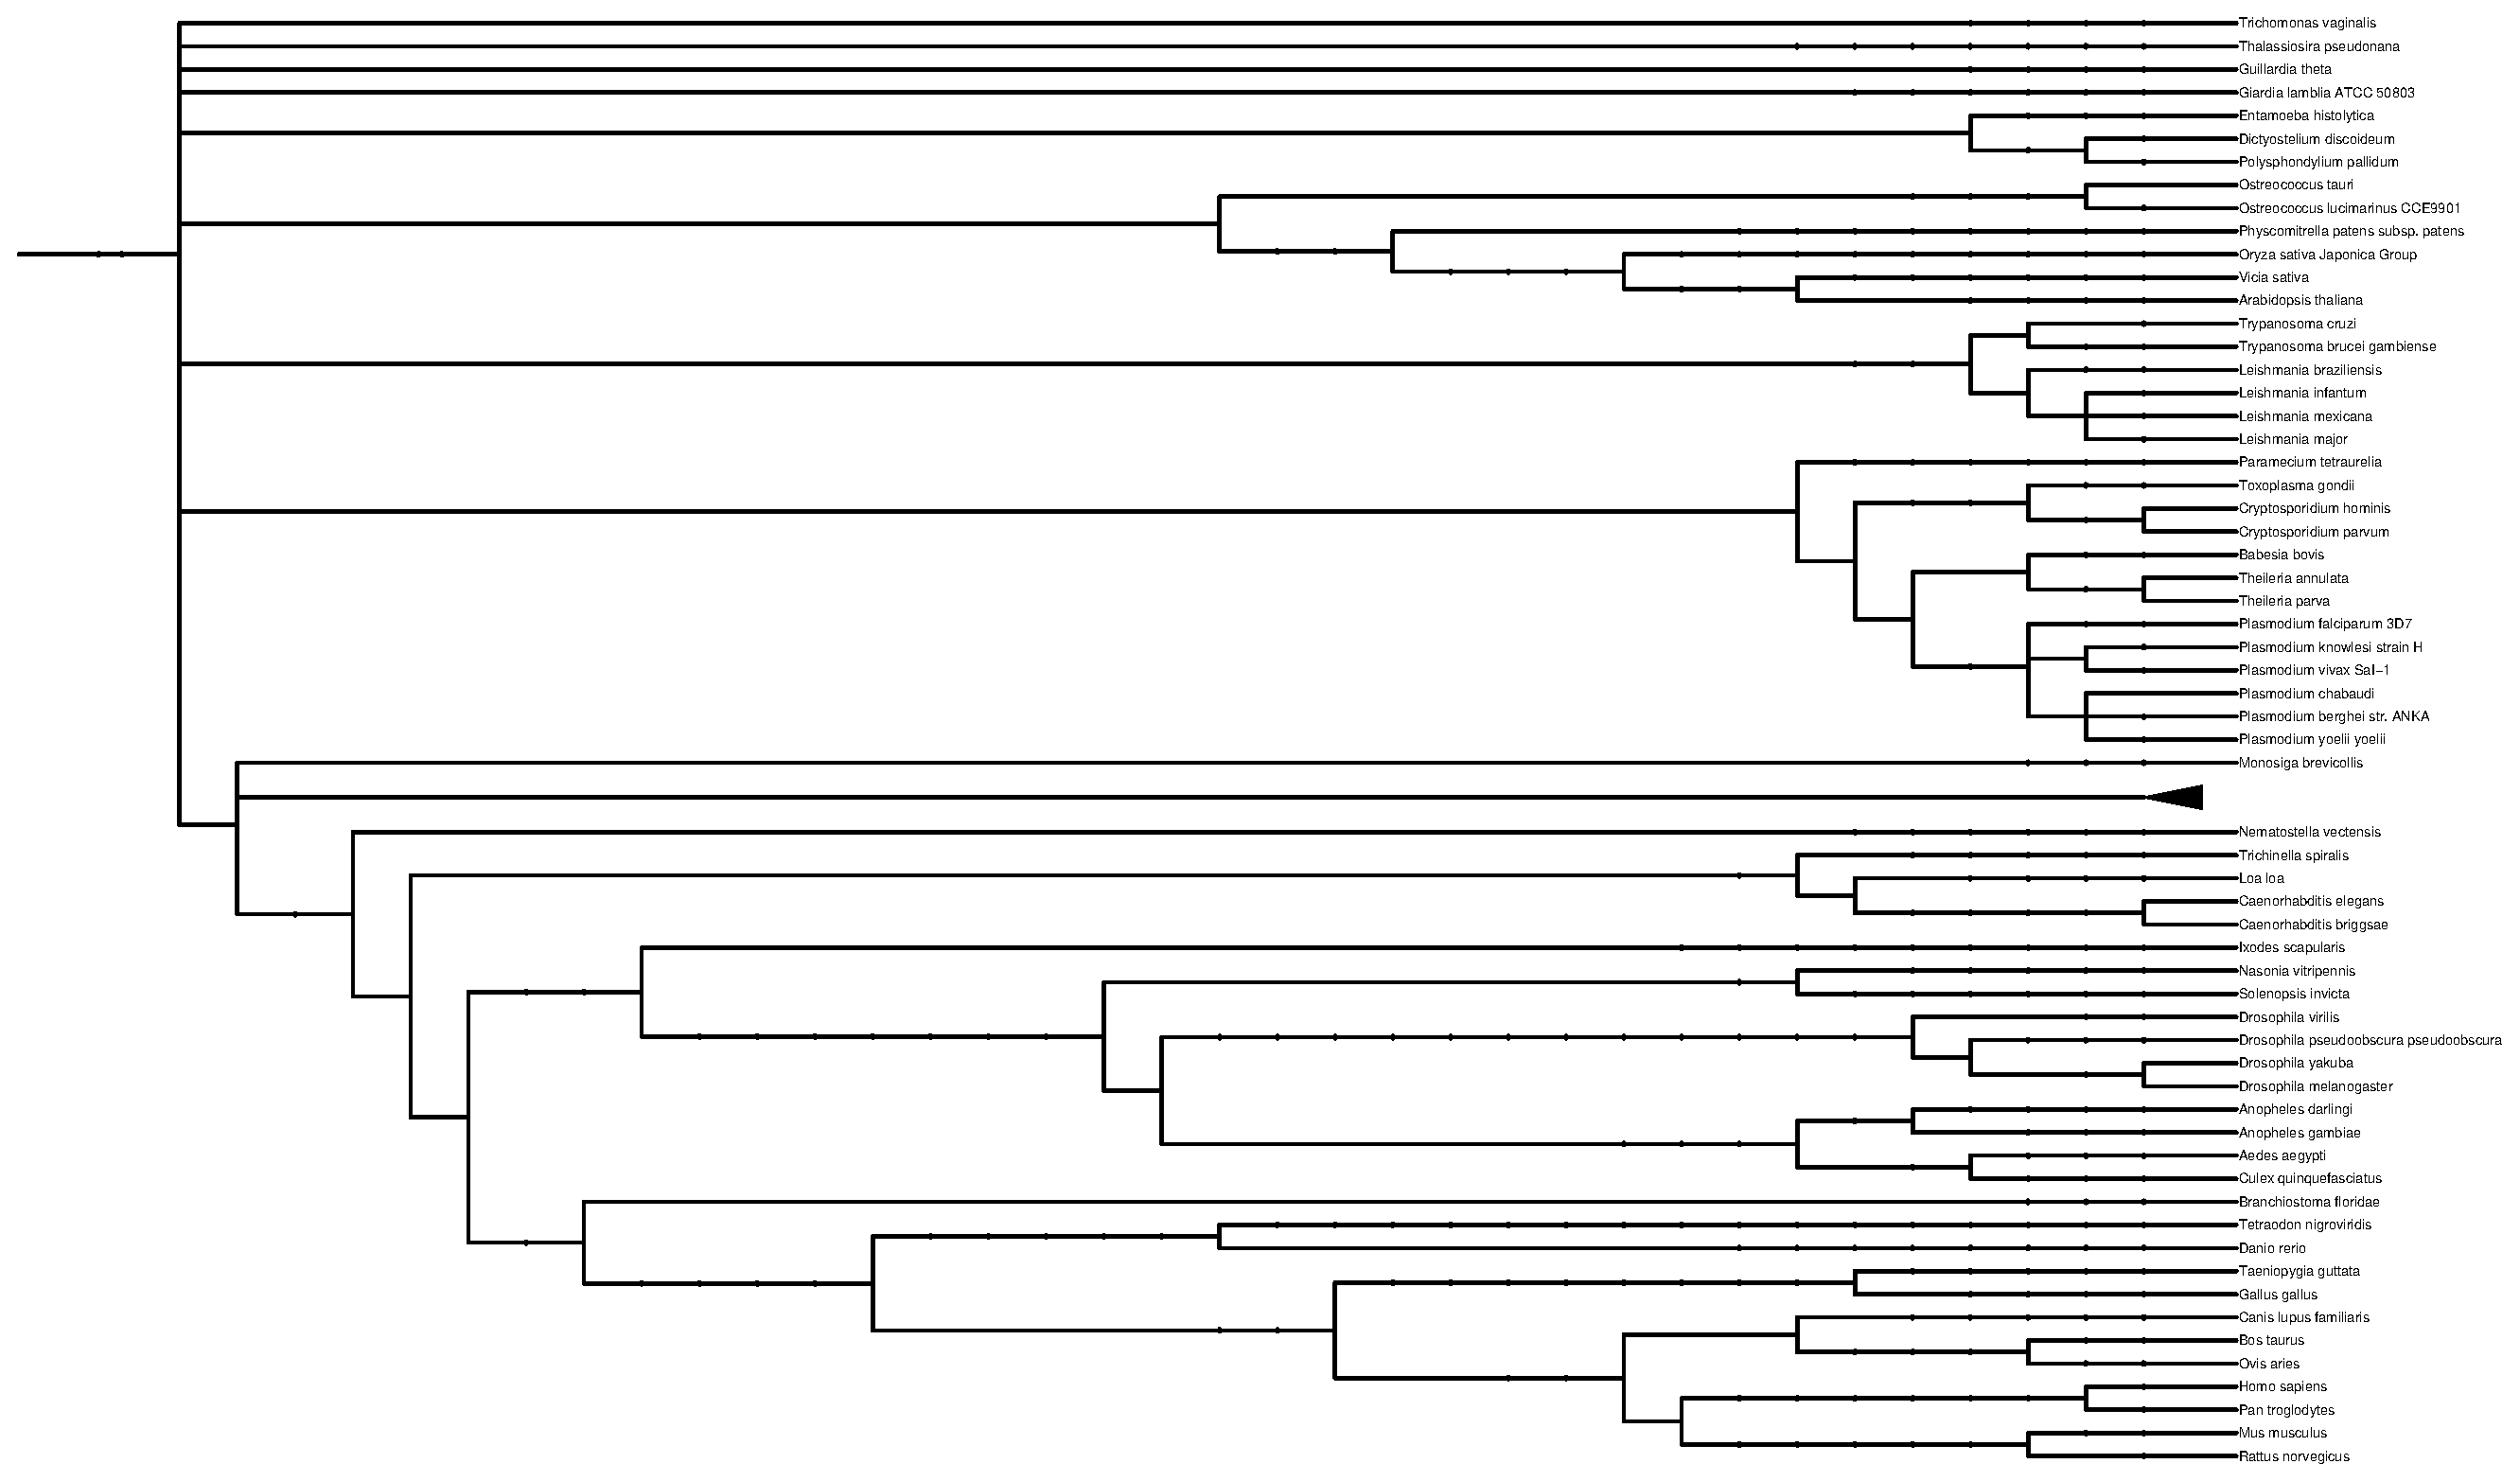
\includegraphics[width=\linewidth]{images/eukaryota1Tree}
  \caption{Tree of Eukaryota genomes. For clarity, the Dikarya are indicated by a triangle and shown separately in figure \ref{fig:eukaryota2Tree}. Phylogenetic trees were drawn using the iTOL software \ref{letunic07}.}
  \label{fig:eukaryotaTree}
\end{figure*}

\begin{figure*}[p] 
\centering
    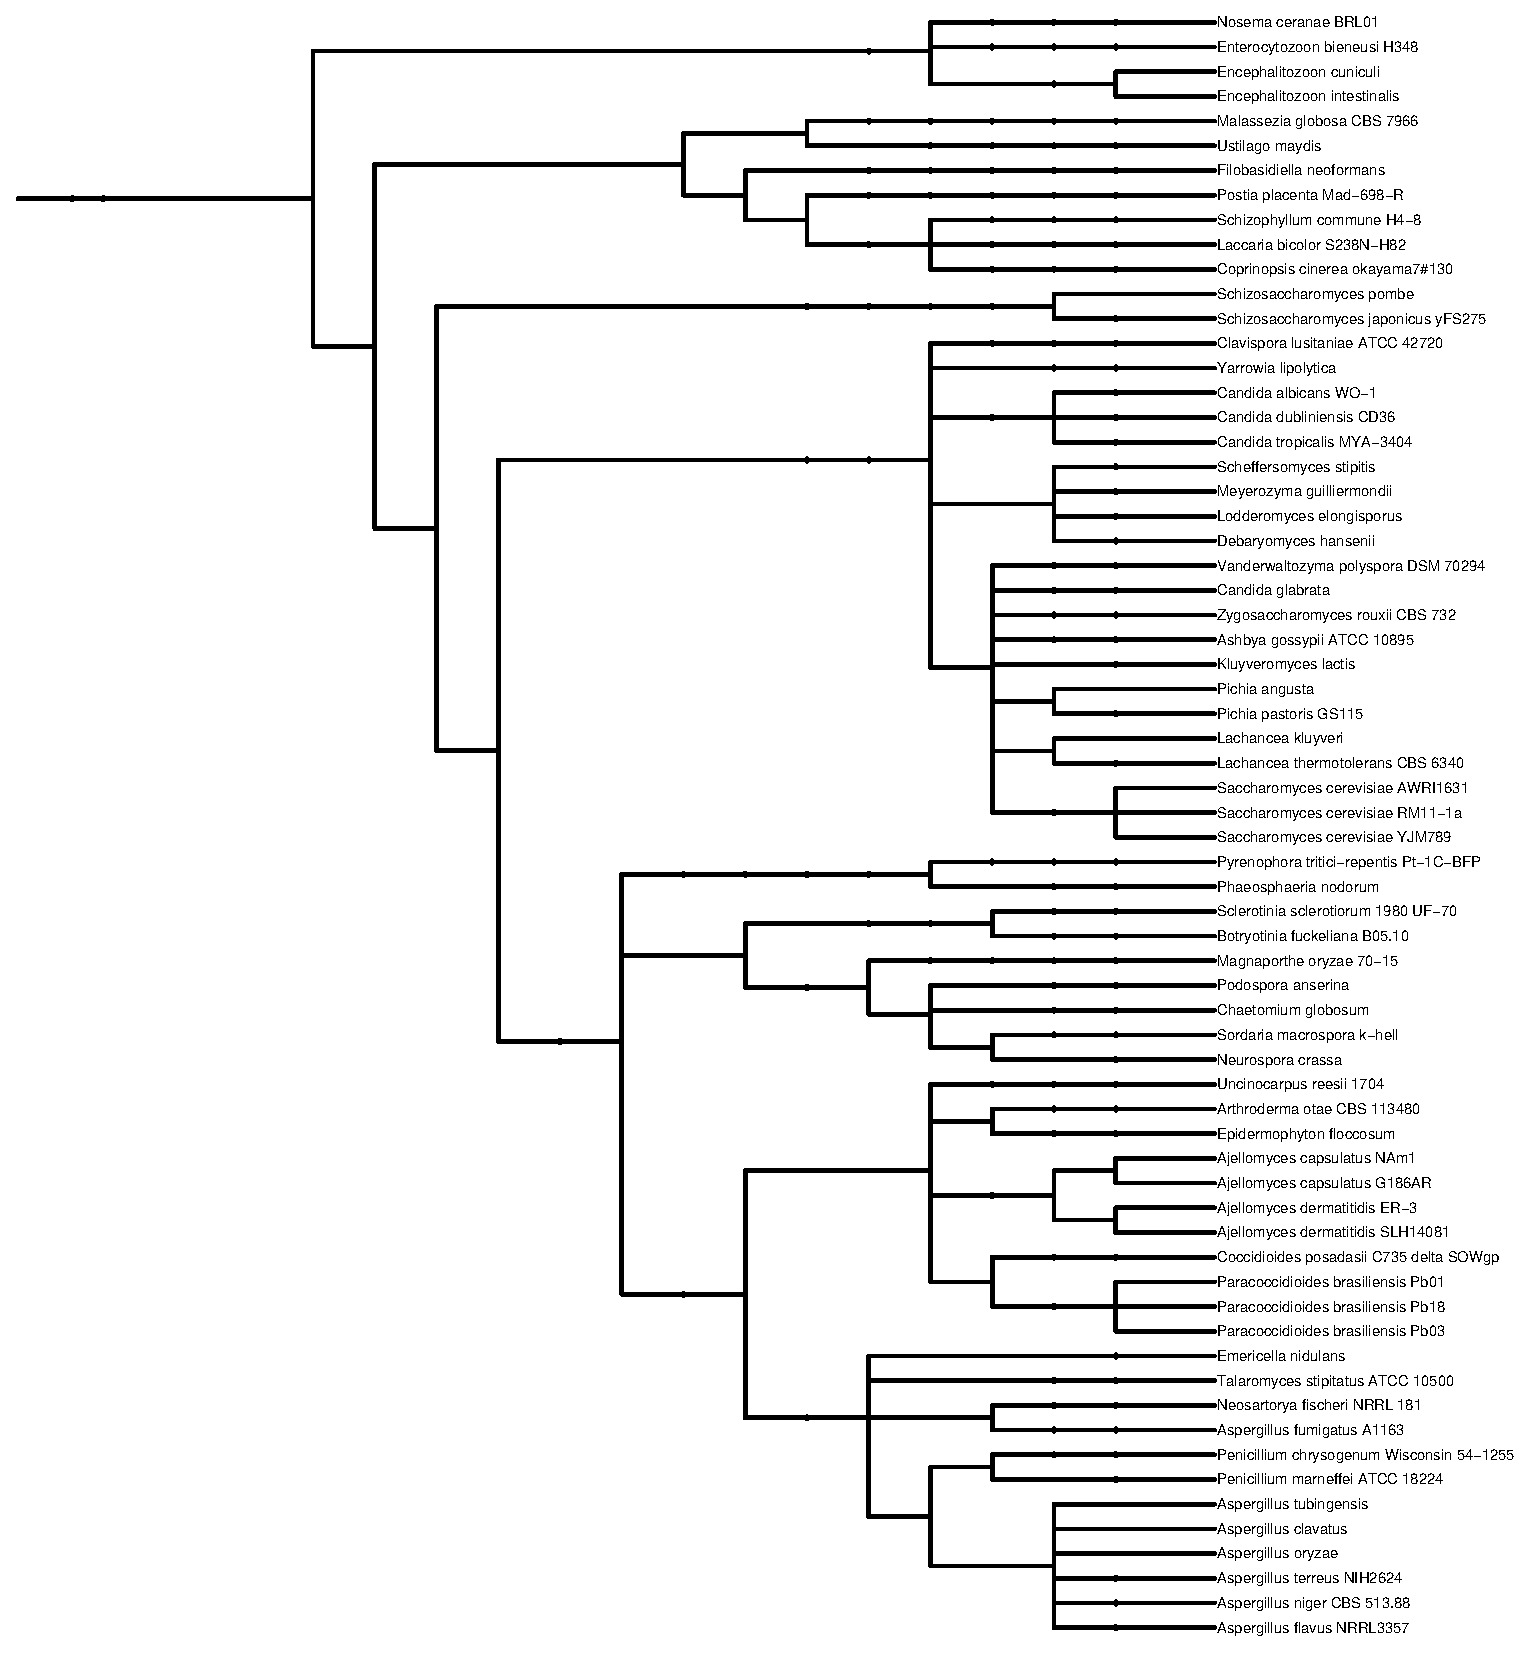
\includegraphics[width=\linewidth]{images/eukaryota2Tree}
  \caption{Subtree of eukaryotes showing Dikarya (higher fungi).}
  \label{fig:eukaryota2Tree}
\end{figure*}

\begin{figure*}[p] 
\centering
    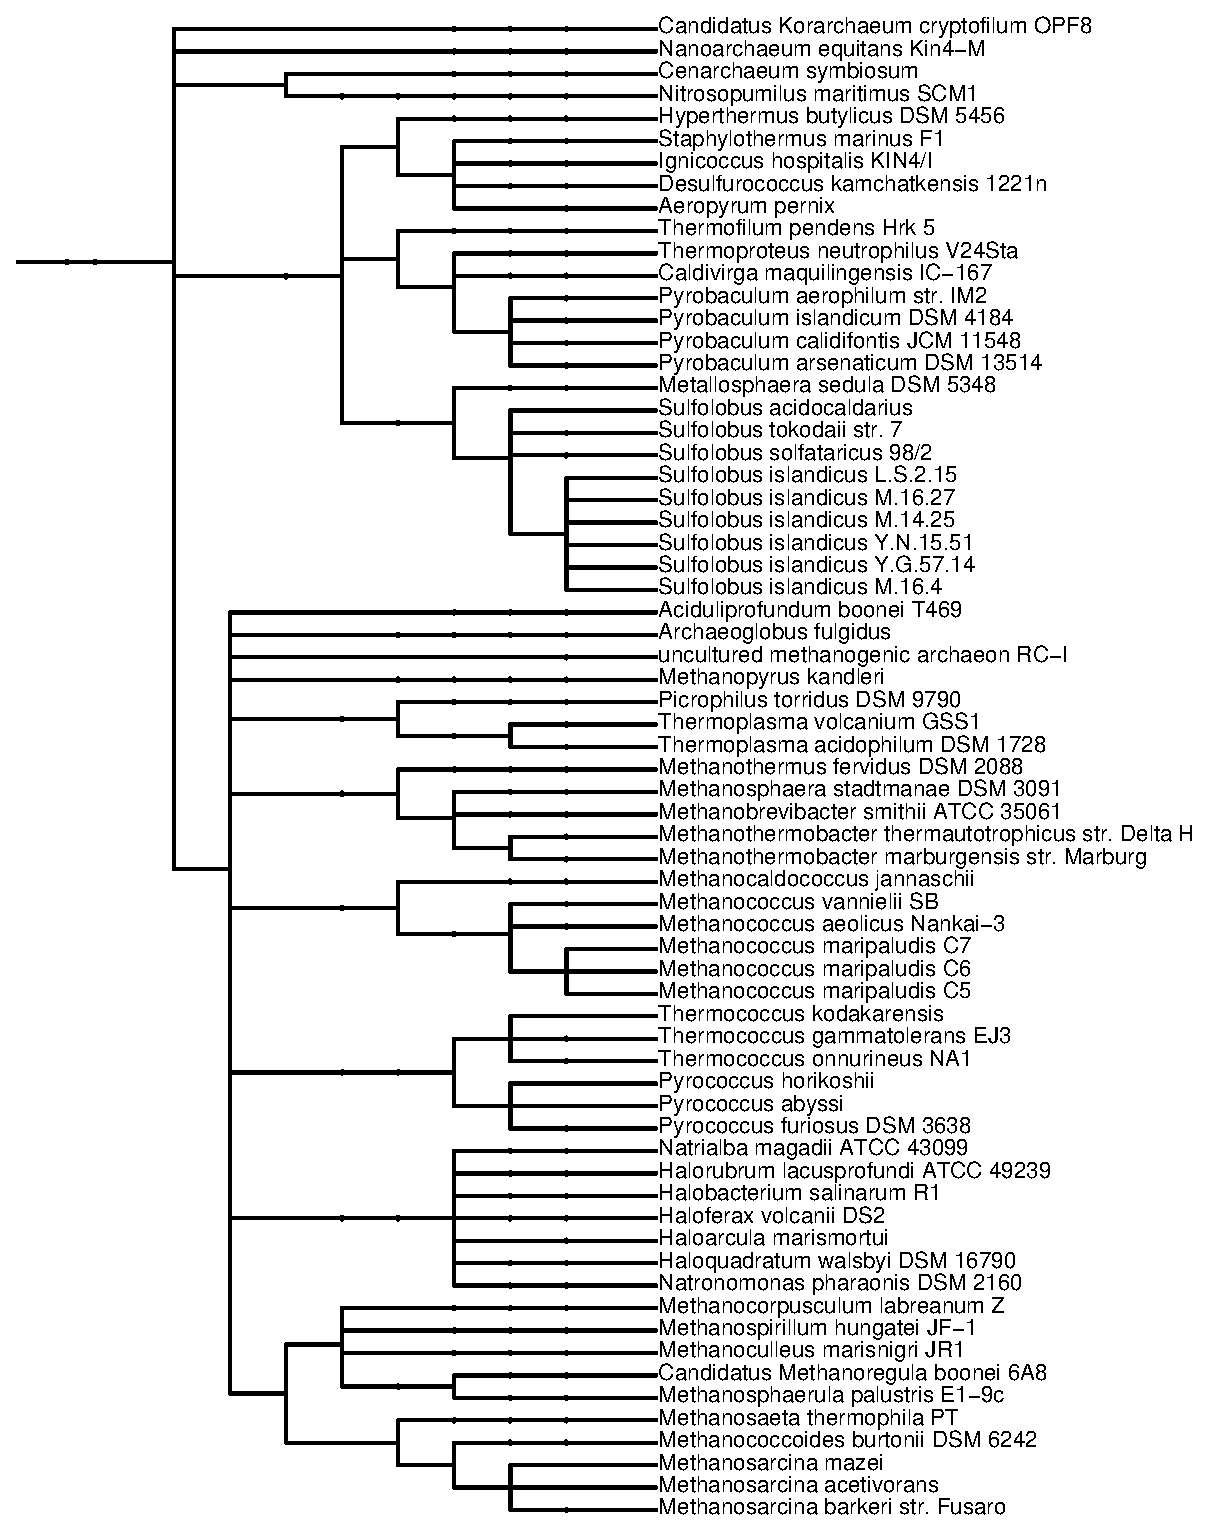
\includegraphics[width=\linewidth]{images/archaeaTree}
  \caption{Tree of Archaea genomes}
  \label{fig:archaeaTree}
\end{figure*}

\begin{figure*}[p] 
\centering
    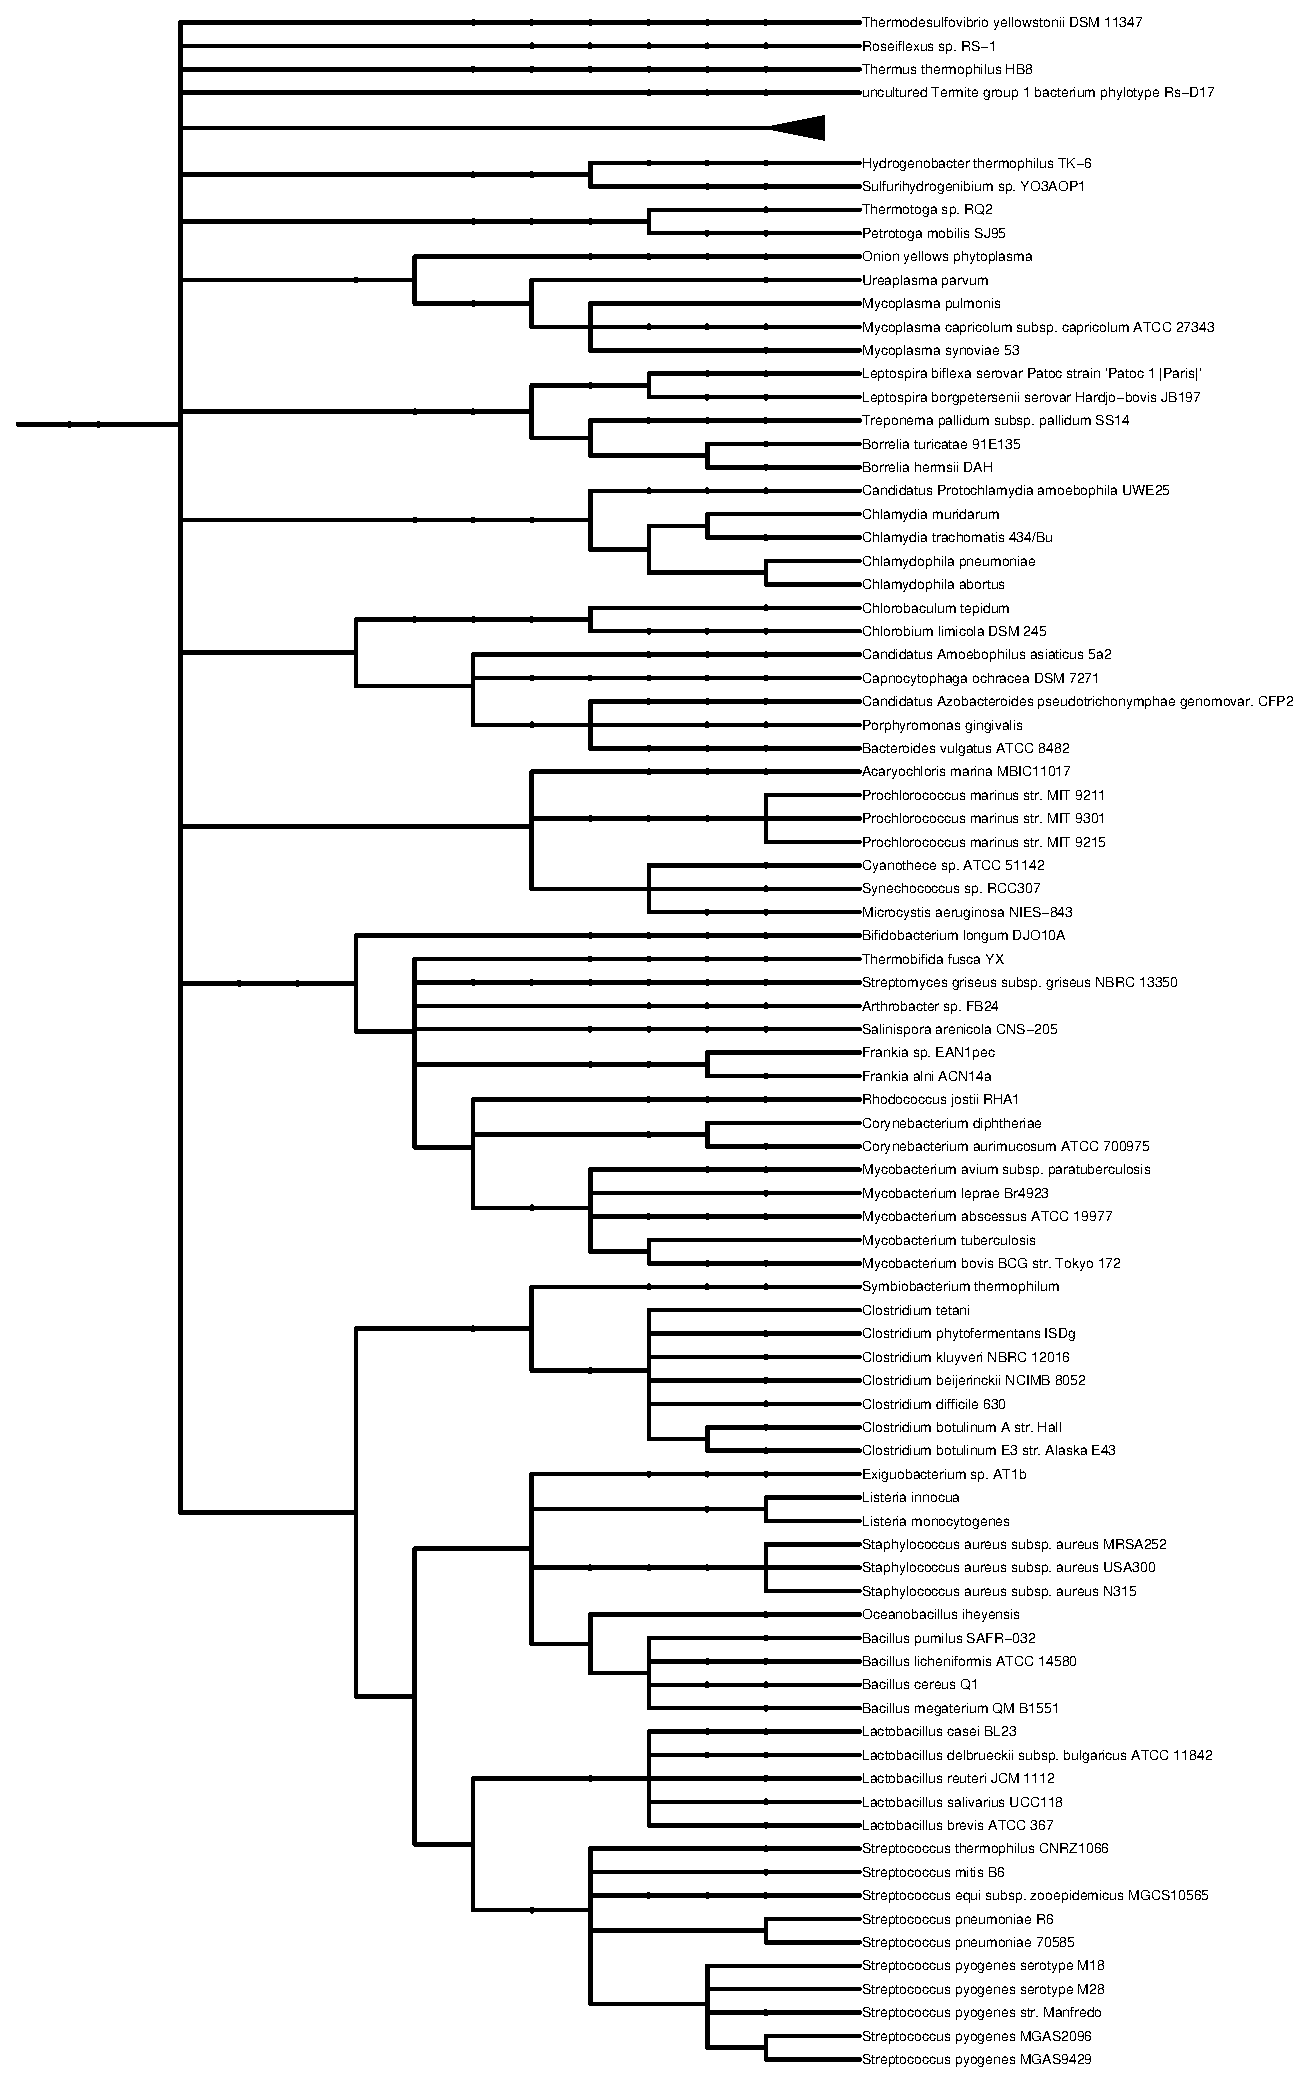
\includegraphics[width=10cm]{images/bacteria1Tree}
  \caption{Partial tree of Bacteria genomes. For clarity, the proteobacteria are indicated by a triangle and shown separately in figure \ref{fig:bacteria2Tree}.}
  \label{fig:bacteriaTree}
\end{figure*}

\begin{figure*}[p] 
\centering
    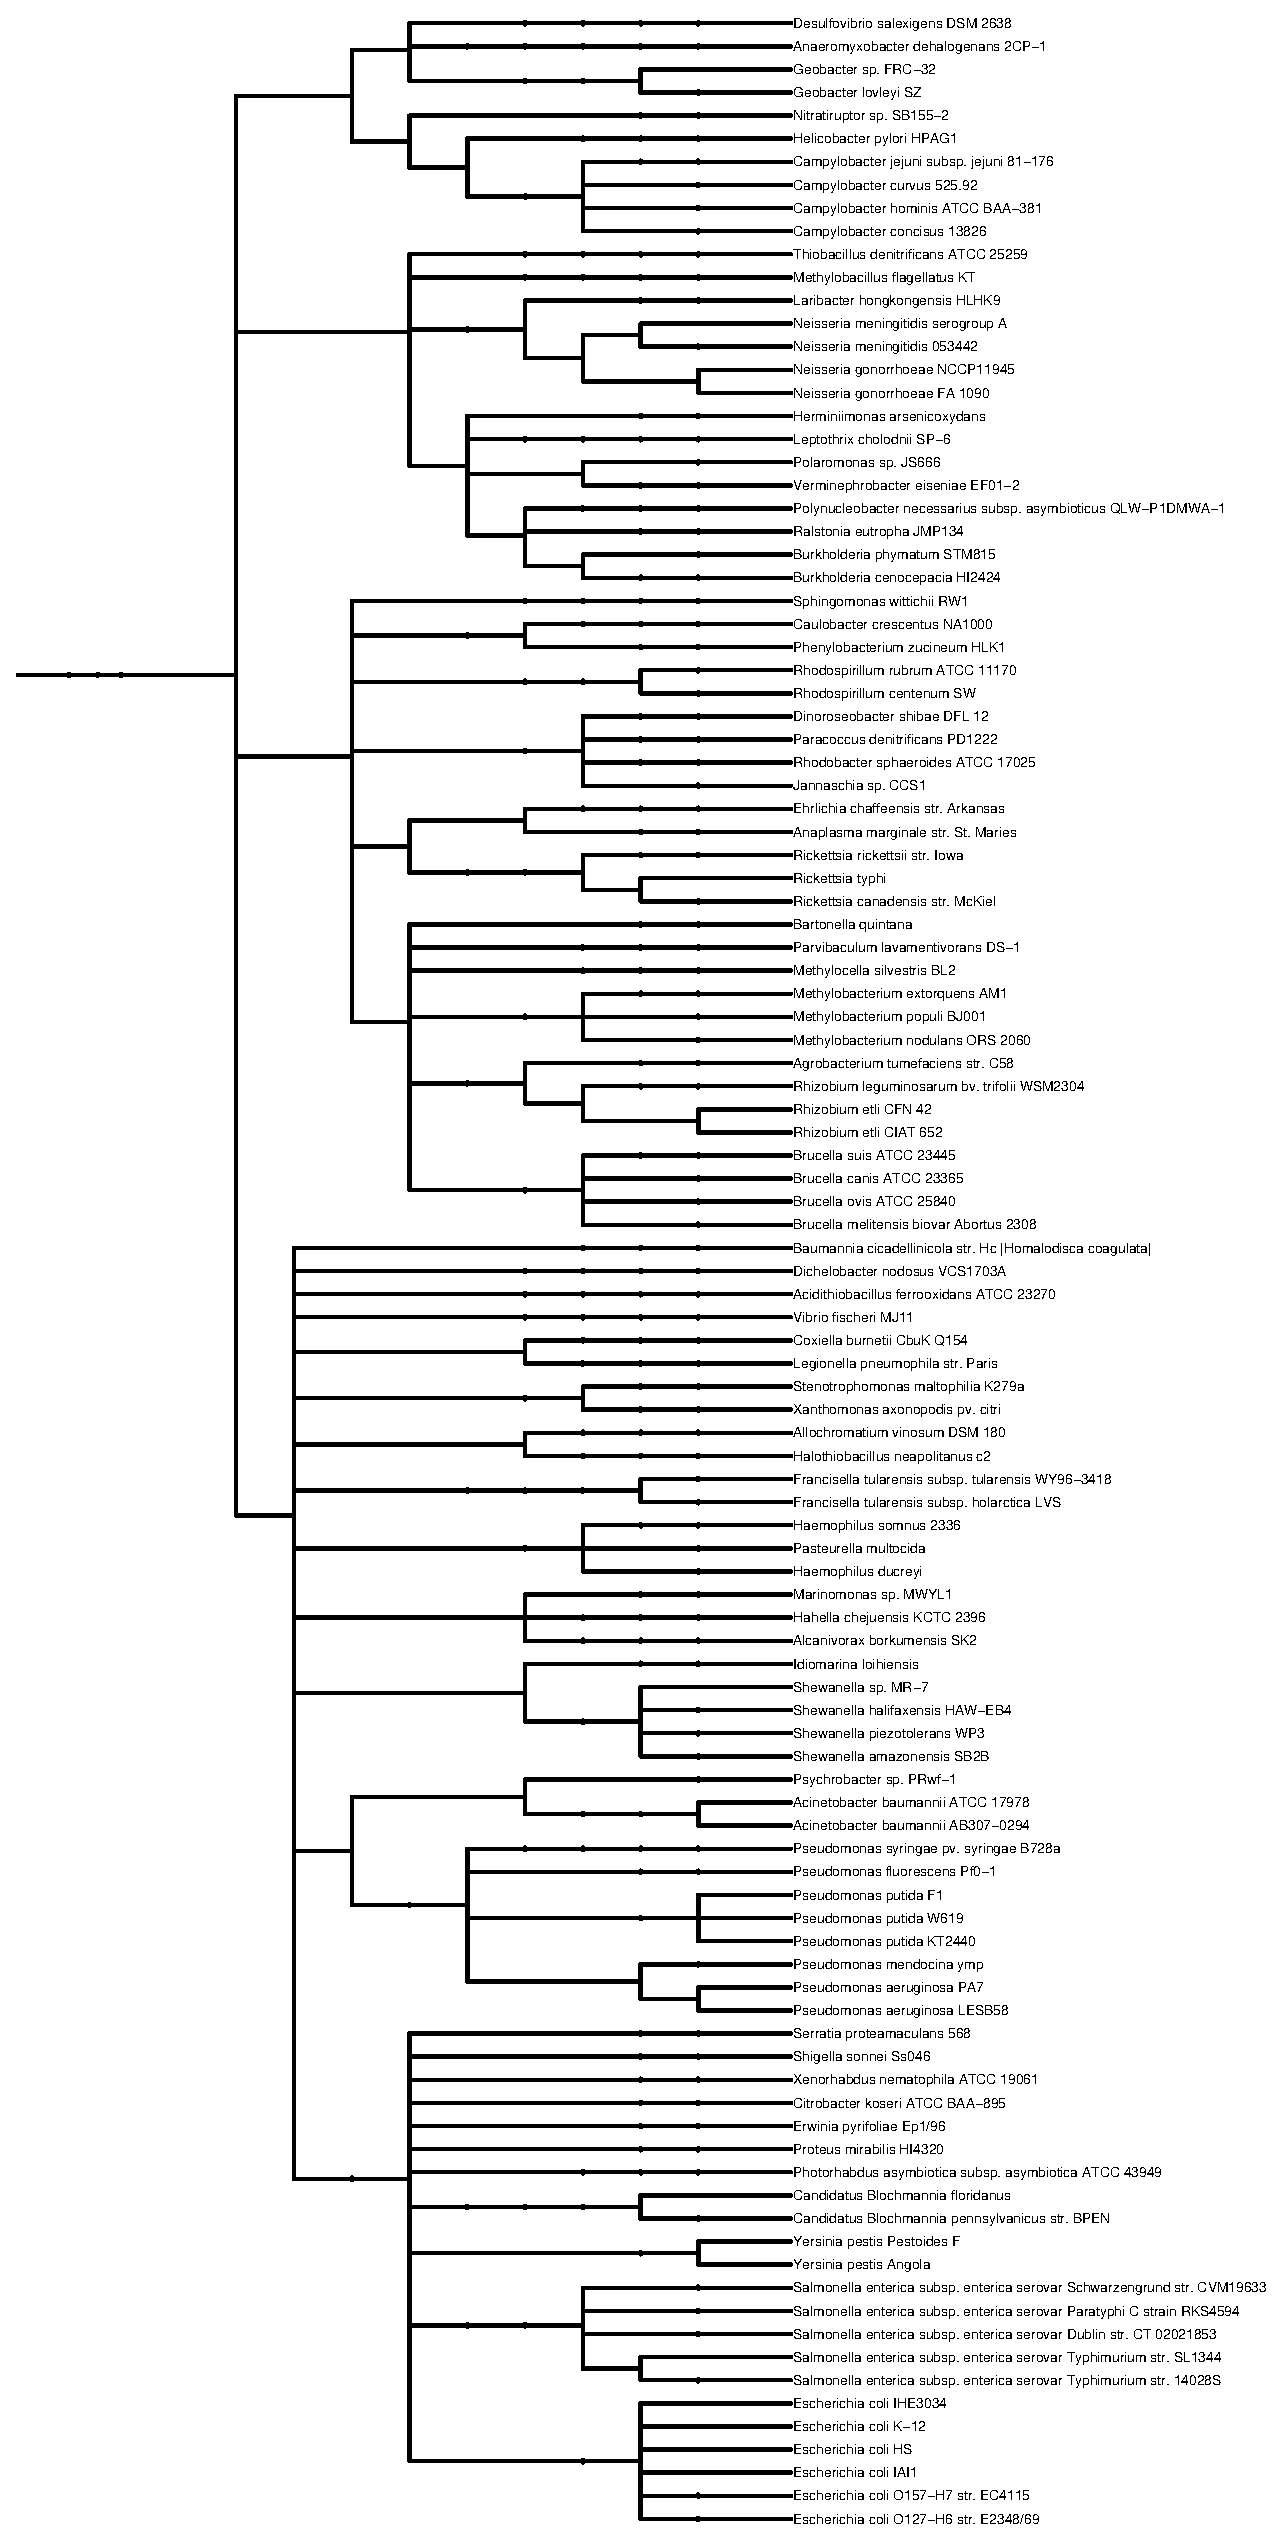
\includegraphics[width=10cm]{images/bacteria2Tree}
  \caption{Partial tree of Bacteria showing Proteobacteria.}
  \label{fig:bacteria2Tree}
\end{figure*}





\nocite{blei02,elkan11,bishop06, heinrich, letunic07, jain, griffiths, finn, bairoch}




{\small
\bibliographystyle{ieee}
\bibliography{egbib}
}
\end{document}
